\section{Aufbau, Durchführung und Auswertung}

\subsection{Charakterisierung des Pumplasers}


\subsubsection{Aufbau und Durchführung}

\begin{figure}[H]
\begin{center}
  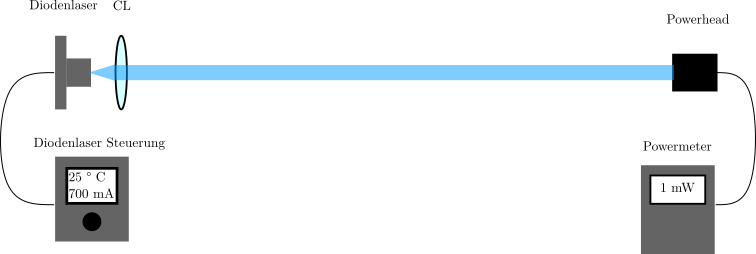
\includegraphics[width=\textwidth]{Aufbau1.png}
  \caption{Schematische Darstellung des Versuchsaufbaus zur Charakterisierung des Pumplasers. Eine
  Linse mit einer Brennweite von 4.6\,mm (CL) wird im Abstand der Brennweite hinter dem Diodenlaser
  platziert, sodass der Laserstrahl dahinter kollimiert ist. In den kollimierten Strahl wird
  anschließend ein Powerhead gestellt, welcher an ein Powermeter angeschlossen ist.}
  \label{img:aufbau1}
\end{center}
\end{figure}

Zur Charakterisierung des Pumplasers verwendeten wir den in Abbildung \ref{img:aufbau1}
dargestellten Aufbau. Die Wellenlänge des verwendeten Diodenlasers beträgt 444\,nm und lässt sich
laut Versuchsanleitung über die Temperatur um 0.05\,nm/\grad und über den Strom um 3.3\,nm/A
verändern \cite{Versuchsanleitung}. Der Laser ist auf einem Peltier-Element montiert und mit einem
Laserdioden Controler verbunden, über den sich die Temperatur zwischen 10\grad und 50\grad und der Strom zwischen 0\,A und
1.4\,A variieren lassen. Um die thermische Last zu verringern, wird der Laser ab einem Strom von
700\,mA automatisch mit einem An-Aus-Verhältnis von 50\,\% und einer Frequenz von 88\,Hz moduliert.
Mit dem verwendeten Powerhead PM 10 (bis 10\,W), welcher mit einem COHERENT Field Mate Powermeter
verbunden ist, wurde die Leistung des kollimierten Pumplasers in 50\,mA Schritten von 0\,A bis
1.4\,A für 25\grad und 35\grad gemessen.


\subsubsection{Auswertung}

\begin{figure}[H]
\begin{center}
  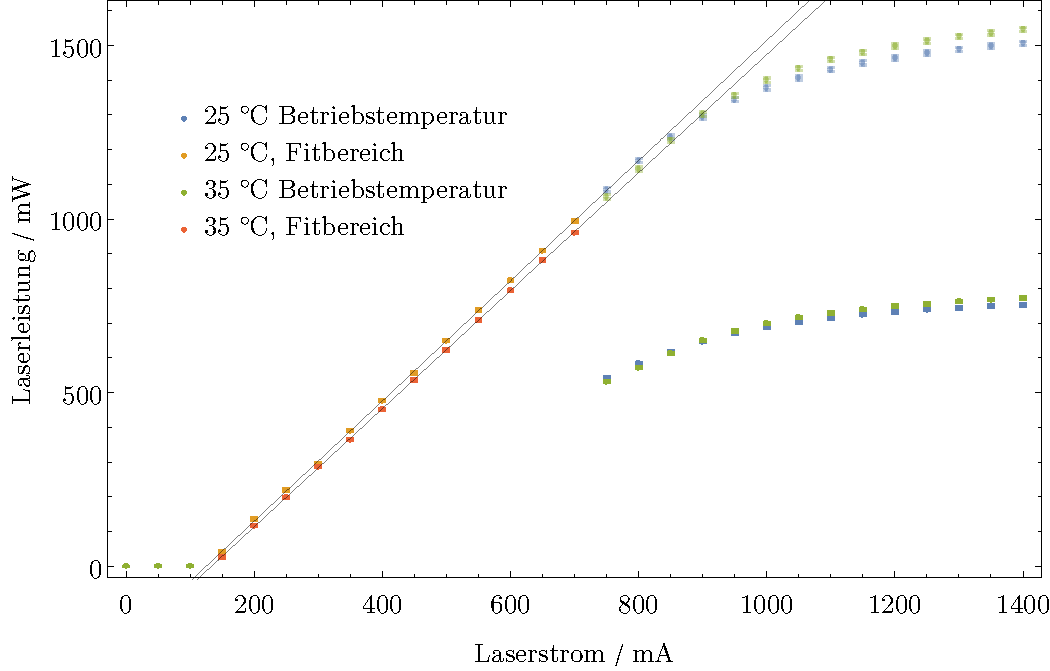
\includegraphics[width=\textwidth]{PI_blau.pdf}
  \caption{PI-Kennlinie des blauen Pumplasers bei 25\grad und 35\grad
  Betriebstemperatur. Der modulationsfreie Bereich wurde mit $y=a(x-b)$
  gefittet, um die Laserschwelle~$b$ und die Effizienz~$a$ zu bestimmen. Im
  Bereich der Modulation mit einer Pulsweite von 50\,\% über 700\,mA Laserstrom ist durch eine
  Multiplikation mit Faktor 2 angedeutet, bei welcher Leistung der Laser
  transient betrieben wird.}
  \label{img:PI_blau}
\end{center}
\end{figure}

Abbildung \ref{img:PI_blau} zeigt die beiden Kennlinien, die bei 25\grad und 35\grad Lasertemperatur
aufgenommen wurde.
Der Fehler der Laserleistung wurde aus der minimalen und maximalen Leistung abgeschätzt, die für die
einzelnen Messpunkte gemessen wurde.
Diese Schwankungen wurden mit höherem Betriebsstrom stärker.
Der Fehler auf den Laserstrom wird als vernachlässigbar klein angenommen.

 Nur der modulationsfreie Bereich von der Laserschwelle bis 700\,mA Laserstrom
zeigt einen linearen Verlauf.
Deshalb wurde der lineare Fit auf diesen Bereich beschränkt.
Da die Modulation des Lasers mit einer Pulsweite von 50\,\% stattfindet, hätte mit einer
Verdoppelung der Leistungen im Bereich über 700\,mA eine Erweiterung des Fitbereichs bis ca. 850\,mA
durchgeführt werden können. Erst bei Betriebsströmen über 850\,mA geht die Leistung deutlich in
Sättigung.
Tabelle \ref{tab:Fits_PI_blau} zeigt die Ergebnisse der beiden Fits.


\begin{table}[htb]
\caption{Ergebnisse der Fits der PI-Kennlinien des Pumplasers mit $y=a(x-b)$ von 150\,mA bis
700\,mA Laserstrom.}
\begin{center}
\begin{tabular}{|c|c|}
\hline
\textbf{25\grad} &  \\ \hline
$a$ & 1.730\,$\pm$\,0.005\,mW\,/\,mA \\ \hline
$b$ & 124.7\,$\pm$\,1.0\,mA \\ \hline
\textchi$^2$ & 16.0142 \\ \hline
\textchi$^2$/\,DoF & 1.60142 \\ \hline
 &  \\ \hline
\textbf{35\grad} &  \\ \hline
$a$ & 1.699\,$\pm$\,0.005\,mW\,/\,mA \\ \hline
$b$ & 133.0\,$\pm$\,1.0\,mA \\ \hline
\textchi$^2$ & 7.24023 \\ \hline
\textchi$^2$/\,DoF & 0.724023 \\ \hline
\end{tabular}
\end{center}
\label{tab:Fits_PI_blau}
\end{table}

\FloatBarrier
 